\chapter{Protostellar Disks and Outflows: Theory}
\label{ch:disks_theory}

\marginnote{
\textbf{Suggested background reading:}
\begin{itemize}
\item \href{http://adsabs.harvard.edu/abs/2014prpl.conf..173L}{Li, Z.-Y., et al. 2014, in ``Protostars and Planets VI", ed.~H.~Beuther et al., pp.~173-194}, sections 3-6 \nocite{li14a}
\end{itemize}
\textbf{Suggested literature:}
\begin{itemize}
\item \href{http://adsabs.harvard.edu/abs/2013MNRAS.432.3320S}{Seifried, D., et al., 2013, MNRAS, 432, 3320} \nocite{seifried13a}
\end{itemize}
}

The previous chapter introduced observations of protostellar disks and their outflows. This companion chapter reviews theoretical models of such disks, with particular attention to how they form, why they accrete, and why they launch outflows.

\section{Disk Formation}

\subsection{The Angular Momentum of Protostellar Cores}

To understand why disks form, we must start with the question of the angular momentum content of the gas that will eventually form the star. To determine this observationally, one maps a core in an optically thin tracer and measures the mean velocity on every line of sight through the core. If there is a systematic gradient in the mean velocity, that is indicative of some net rotation. Doing this for a sample of cores yields a distribution of rotation rates.

It is most convenient to express the resulting distribution dimensionlessly, in terms of the ratio of kinetic energy in rotation to gravitational binding energy. If the angular velocity of the rotation is $\Omega$ and the moment of inertia of the core is $I$, this is
\begin{equation}
\beta = \frac{(1/2)I\Omega^2}{a G M^2/R},
\end{equation}
where $a$ is our usual numerical factor that depends on the mass distribution. For a sphere of uniform density $\rho$, we get
\begin{equation}
\beta = \frac{1}{4\pi G \rho}\Omega^2 = \frac{\Omega^2 R^3}{3 G M}
\end{equation}
Thus we can estimate $\beta$ simply given the density of a core and its measured velocity gradient. Observed values of $\beta$ typically a few percent \citep[e.g.,][]{goodman93a}.

This implies that cores are not primarily supported by rotation. In fact, we can understand the observed rotation rates as being a property of the turbulence. Although cores are primarily thermally-supported, they do still have some turbulent motions present at transsonic or subsonic levels. Since most of the power in this turbulence is on large scales, there is likely to be a net gradient. When one performs the experiment of generating random turbulent velocity fields with a variety of power spectra and analyzing them as an observer would, the result is a $\beta$ distribution that agrees very well with the observed one \citep{burkert00a}.

\subsection{Rotating Collapse: the Hydrodynamic Case}

Given this small amount of rotation, how can we expect it to affect the collapse? Let us take the simplest case of a cloud in solid body rotation at a rate $\Omega$. Consider a fluid element that is initially at some distance $\varpi_0$ from the axis of rotation. We will consider it to be in the equatorial plane, since fluid elements at equal radius above the plane have less angular momentum, and thus will fall into smaller radii.

Its initial angular momentum in the direction along the rotation axis is $j=\varpi_0^2\Omega$. If pressure forces are insignificant for this fluid element, it will travel ballistically, and its specific angular momentum and energy will remain constant as it travels. At its closest approach to the central star plus disk, its radius is $\varpi_{\rm min}$ and by conservation of energy its velocity is $v_{\rm max} = \sqrt{2 G m_*/\varpi_{\rm min}}$, where $m_*$ is the mass of the star plus the disk material interior to this fluid element's position.
Conservation of angular momentum them implies that $j=\varpi_{\rm min} v_{\rm max}$.

Combining these two equations for the two unknowns $\varpi_{\rm min}$ and $v_{\rm max}$, we have
\begin{equation}
\varpi_{\rm min} = \frac{\varpi_0^4 \Omega^2}{G m_*} = \frac{4\pi \rho \beta \varpi_0^4}{m_*},
\end{equation}
where we have substituted in for $\Omega^2$ in terms of $\beta$. This tells us the radius at which infalling material must go into a disk because conservation of angular momentum and energy will not let it get any closer.

We can equate the stellar mass $m_*$ with the mass that started off interior to the position of the fluid element we are considering. This amounts to assuming that the collapse is perfectly inside-out, and that the mass that collapses before the fluid element under consideration all makes it onto the star. If we make this approximation, then $m_*=(4/3)\pi \rho \varpi_0^3$, and we have
\begin{equation}
\varpi_{\rm min} = 3 \beta \varpi_0,
\end{equation}
i.e., the radius at which the fluid element settles into a disk is simply proportional to $\beta$ times a numerical factor of order unity.

We should not take the factor too seriously, since of course real clouds are not uniform spheres in solid body rotation, but the result that rotation starts to influence collapse and force disk formation at a radius that is a few percent of the core radius is interesting. It implies that for cores that are $\sim 0.1$ pc in size and have $\beta$ values typical of what is observed, they should start to become rotationally flattened at radii of several hundred AU. This should be the typical size scale of protostellar disks in the hydrodynamic regime.

\subsection{Rotating Collapse: the Magnetohydrodynamic Case}

Magnetic fields can greatly complicate this picture, due to magnetic braking. As a core contracts, conservation of angular momentum causes it to spin faster, but this in turn twists up the magnetic field. This creates a tension force that opposes the rotation, and tries to keep the core rotating as a solid body.

To analyze this effect, let us work in cylindrical coordinates $(\varpi, \phi, z)$. Consider a fluid element in a disk at a distance $\varpi$ from the star, whose dimensions are $d\varpi$, $d\phi$, $dz$ in the $\varpi$, $\phi$, and $z$ directions. The fluid element is rotating around the star with a velocity $v_{\phi}$ in the $\phi$ direction. The fluid element is threaded by a magnetic field $\vecB=(B_\varpi, B_\phi, B_z)$. For future convenience we define the poloidal component of the field to be
\begin{equation}
\vecB_p = (B_\varpi, B_z),
\end{equation}
i.e., it is the component of the field not associated with wrapping around the rotation axis. The $\phi$ component of the field is called the toroidal component, since it represents the part of the field that is wrapped in the rotation direction. To help visualize this, imagine drawing a two-dimensional plot of the system in the $(\varpi, z)$-plane. In this plot, the poloidal component is the one on the page, and the toroidal component is the one going into or out of the page.

We will assume that both the fluid and the magnetic field are axisymmetric, so that they do not vary with $\phi$, although the field does have a $\phi$ component. The magnetic field exerts a Lorentz force per unit volume on the fluid element given by
\begin{eqnarray}
\mathbf{f} & = & \frac{1}{4\pi} \left[(\nabla\times\vecB)\times \vecB\right] \\
& = & \frac{1}{4\pi} \left[\frac{B_\varpi}{\varpi} \frac{\partial(\varpi B_\phi)}{\partial \varpi} + B_z  \frac{\partial B_\phi}{\partial z}\right] \hat{\phi}\\
& = & \frac{1}{4\pi\varpi} \vecB_p \cdot \nabla_p (\varpi B_{\phi}) \hat{\phi},
\end{eqnarray}
where all the components except the $\phi$ one vanish by symmetry, and in the final step we have defined the poloidal gradient as $\nabla_p = (\partial/\partial\varpi, \partial/\partial z)$, i.e., it is just the components of the gradient in the $\varpi$ and $z$ directions.

The rate of change of the momentum associated with the Lorentz force alone is
\begin{equation}
\frac{\partial}{\partial t}(\rho \vecv) = \mathbf{f},
\end{equation}
so writing down the $\phi$ component of this equation and multiplying on both sides by $\varpi$, we have
\begin{equation}
\frac{\partial}{\partial t} (\rho v_{\phi} \varpi) = \frac{1}{4\pi} \vecB_p\cdot\nabla_p(\varpi B_\phi)
\end{equation}
The left hand side of this equation just represents the time rate of change of the angular momentum per unit volume $\rho v_{\phi} \varpi$, while the right hand side represents the torque per unit volume exerted by the field.

Given this equation, how quickly can a magnetic field stop rotation? We can define a magnetic braking time by
\begin{equation}
t_{\rm br} = \frac{\rho v_{\phi} \varpi}{\frac{\partial}{\partial t} (\rho v_{\phi} \varpi)}
= \frac{4 \pi \rho v_{\phi} \varpi}{\vecB_p \cdot\nabla_p (\varpi B_\phi)}
\end{equation}
To evaluate this timescale, consider the case of a fluid element that is part of a collapsing cloud, and is trying to rotate at a velocity $v_{\phi}$ equal to the Keplerian velocity, i.e.,
\begin{equation}
v_{\phi} = \sqrt{\frac{GM}{\varpi}},
\end{equation}
where $M$ is the mass interior to the fluid element.

If we started with a uniform cloud of density $\rho$, the mass interior to our element is $M\approx (4\pi/3) \rho \varpi^3$, so $v_\phi \approx \sqrt{(4\pi/3) G \rho \varpi^2}$. Plugging this into the timescale, we have
\begin{equation}
t_{\rm br} \approx \frac{(4\pi \rho)^{3/2} G^{1/2} \varpi^2}{\vecB_p \cdot\nabla_p (\varpi B_\phi)}.
\end{equation}

To make an order of magnitude estimate of what this implies, let us suppose that the poloidal and toroidal components of the field are comparable, and that the characteristic length scale on which the field varies is $\varpi$, so the field is fairly smooth on all scales smaller than the size of the region that is currently collapsing. In this case $\vecB_p \cdot \nabla_p (\varpi B_\phi) \sim B^2$, so the time scale becomes
\begin{eqnarray}
t_{\rm br} & \sim & \frac{G^{1/2}\rho^{3/2} \varpi^2}{B^2} \\
& \sim & \frac{(G\rho)^{1/2} \varpi^2}{v_A^2} \\
& \sim & \frac{t_{\rm cr}^2}{t_{\rm ff}},
\end{eqnarray}
where we are dropping constants of order unity. Note that in the second step we wrote $B$ in terms of the Alfv\'en speed $v_A = B/\sqrt{4\pi \rho}$, and in the final step we wrote $t_{\rm cr} = \varpi/v_A$, where $t_{\rm cr}$ is the Alfv\'en crossing time of the cloud.

If a cloud starts out with a magnetic field near equipartition with gravity and thermal energies, we expect $t_{\rm ff} \sim t_{\rm cr}$, so this means that $t_{\rm br}\sim t_{\rm cr}$. This is an order of magnitude calculation, but its implication is clear: if we have a field that is even marginally wound up, such that the poloidal and toroidal components become comparable, this field is capable of stopping Keplerian rotation in a time scale comparable to the collapse or crossing time. This can effectively prevent formation of a Keplerian disk at all if the magnetic field is strong enough. Indeed, this is what simulations seem to show happening (Figure \ref{fig:magdisk_hennebelle}).

\begin{marginfigure}
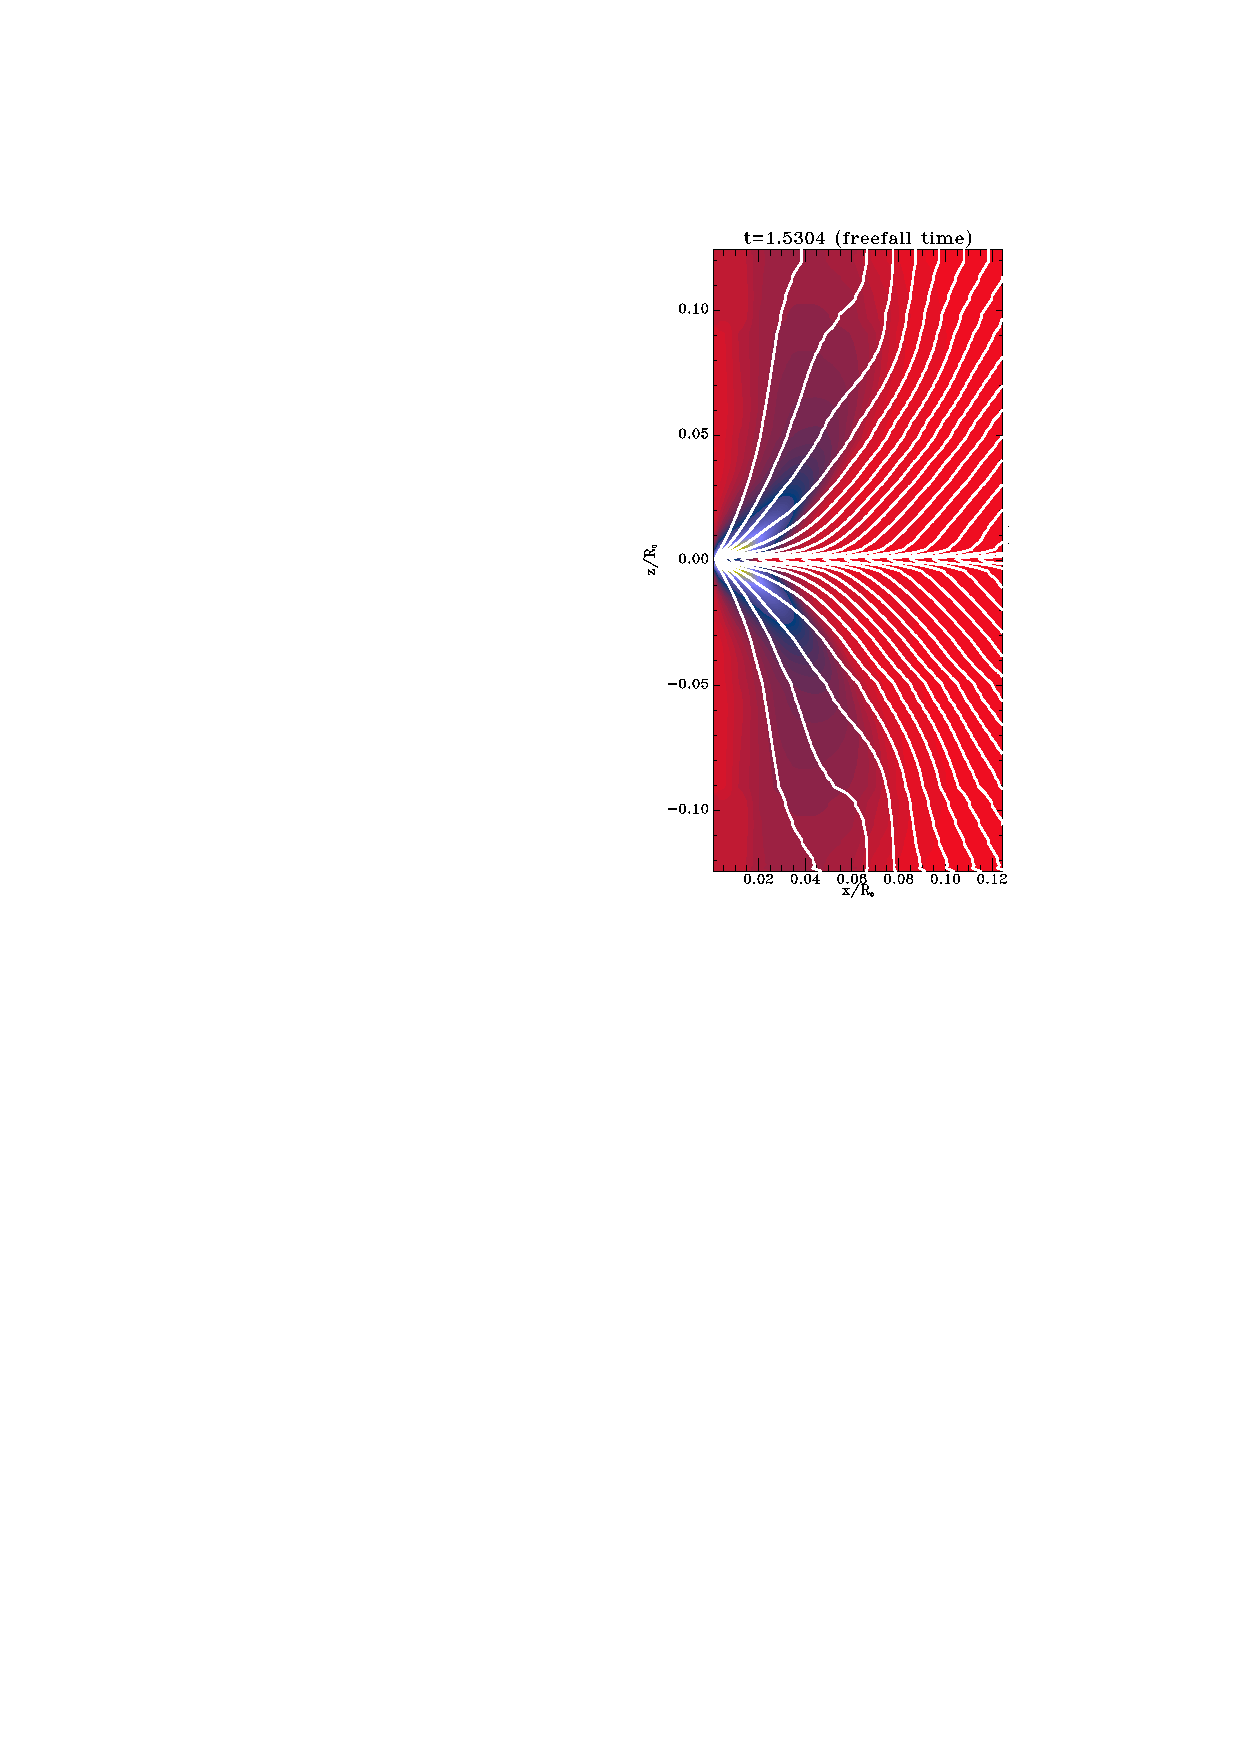
\includegraphics[width=\linewidth]{magdisk1_hennebelle08}
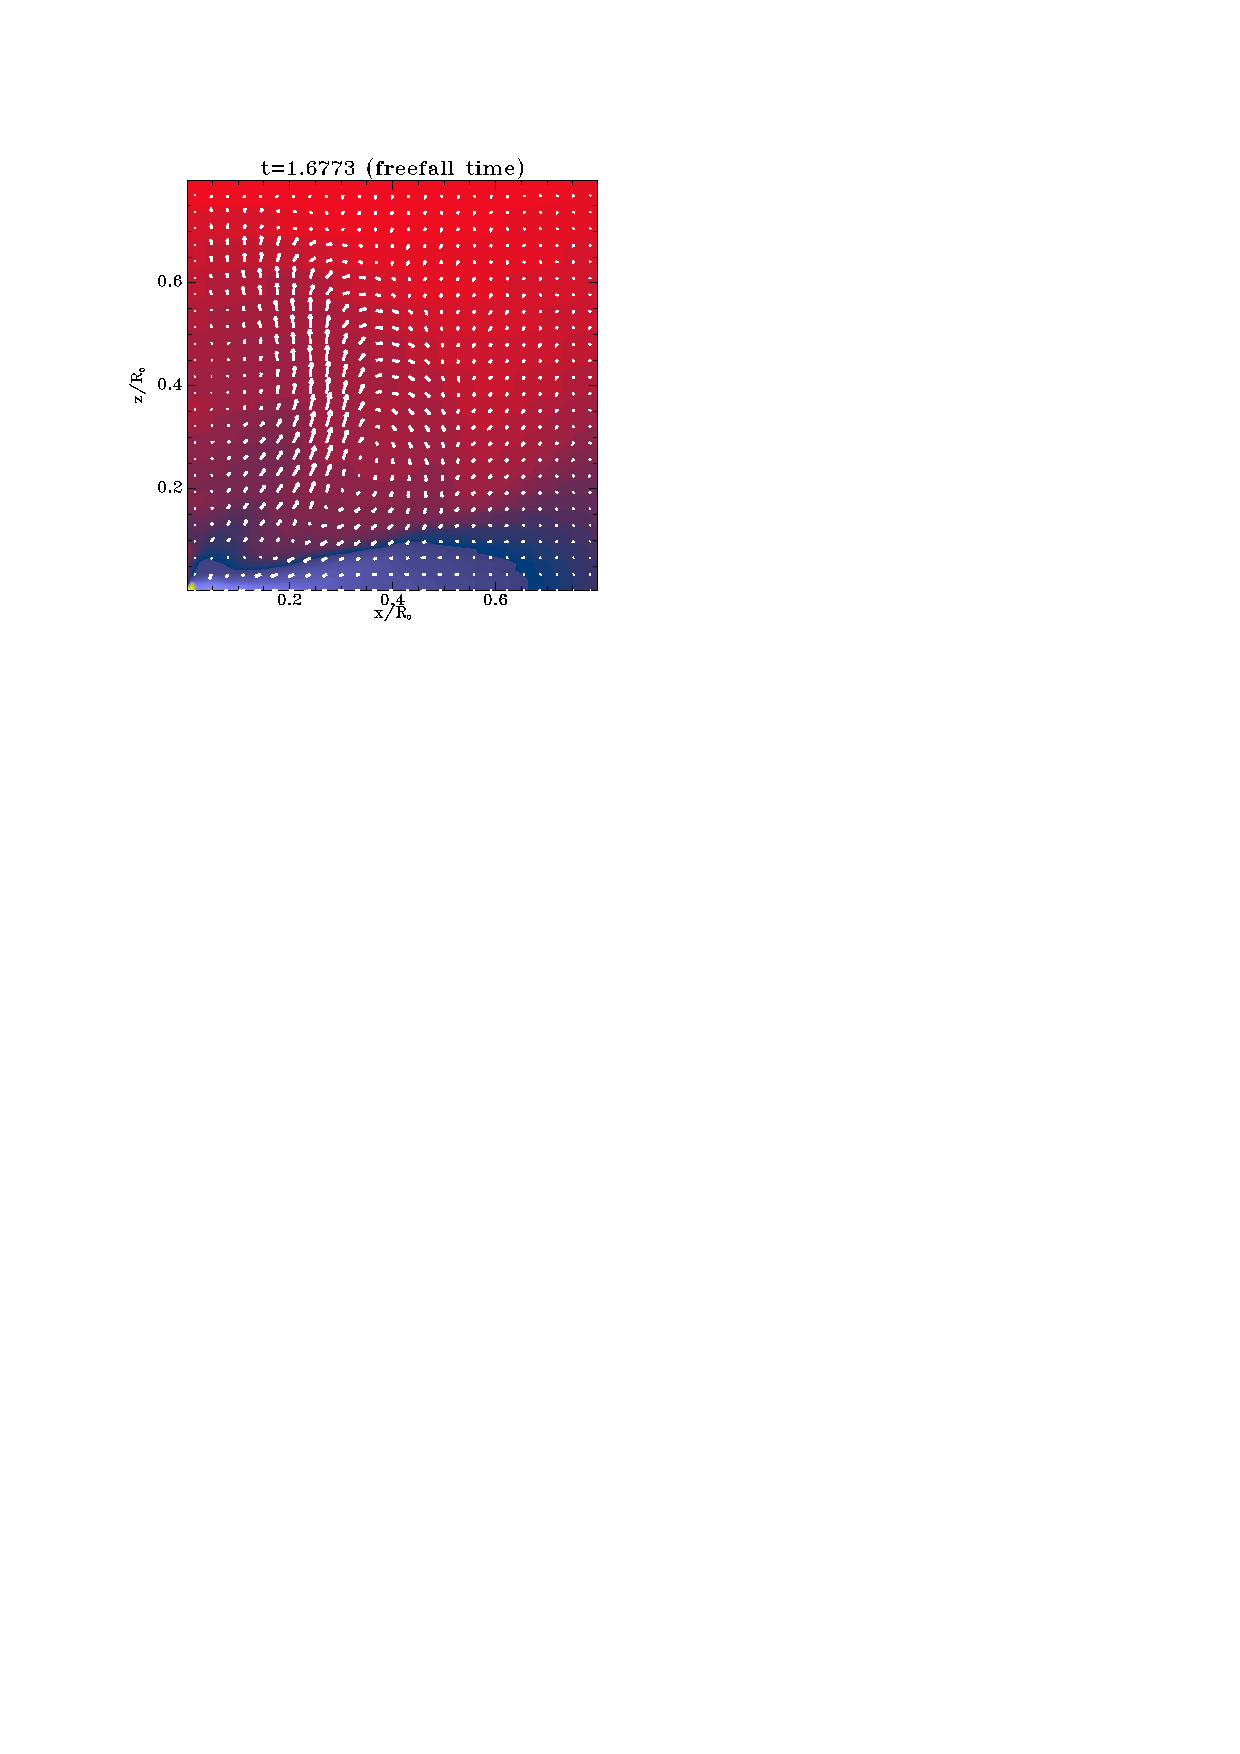
\includegraphics[width=\linewidth]{magdisk2_hennebelle08}
\caption[Simulations of magnetized rotating collapse]{
\label{fig:magdisk_hennebelle}
Results from a simulation of magnetized rotating collapse. The top panel shows the magnetic field structure; solid lines are poloidal magnetic field lines, while color indicates the azimuthally-averaged total magnetic field strength, on a scale from $0-3.5$ mG. The bottom panel shows the density (color) and velocity (arrows) structure at a slightly later time in the simulation. The structure in the mid-plane is a non-rotating pseudo-disk. Credit:  \citeauthor{hennebelle08c}, A\&A, 477, 9, 2008, reproduced with
permission \copyright\,ESO.
}
\end{marginfigure}

\subsection{The Magnetic Braking Problem and Possible Solutions}

The calculation of magnetic braking we have just performed presents us with a fundamental problem: it naively seems like magnetic fields should prevent disks from forming at all, but we observe that they do. We even observe disks present in class 0 sources, where the majority of the gas is still in the envelope. So how can we get out of this? This is not a completely solved problem, but we can make a few observations about what a solution might look like.

We can first ask whether ion-neutral drift might offer a way out. Recall in Chapter \ref{ch:magnetic}, we showed that, at the densities and velocities typical of protostellar cores, ion-neutral drift should allow gas to decouple from the magnetic field on scales below $L_{\mathrm{AD}} \sim 0.05$ pc. One might expect that this would make it possible to form disks below the decoupling scale. However, simulations suggest that this solution does not work. The flux that is released from the gas by ion-neutral drift does not disappear. Instead, it builds up flux tubes near the star with relatively little mass on them, and these flux tubes prevent a disk from forming (Figure \ref{fig:magdisk_krasnopolsky12}).

A more promising solution appears to be misalignment between the rotation axis of the gas and the magnetic field, or, more generally, the presence of turbulence in the collapsing gas. In simulations where the gas is turbulent, the magnetic field lines tend to be bent or misaligned relative to the disk, and this greatly reduces the efficiency of magnetic braking. However, the problem of how disks form is still not fully solved.

\section{Disk Evolution}

Given that disks do exist, in the real universe if not in our models, we wish to understand how they evolve, and how they accrete onto their parent stars. We therefore sketch here a basic theory for how disks behave.

\begin{marginfigure}
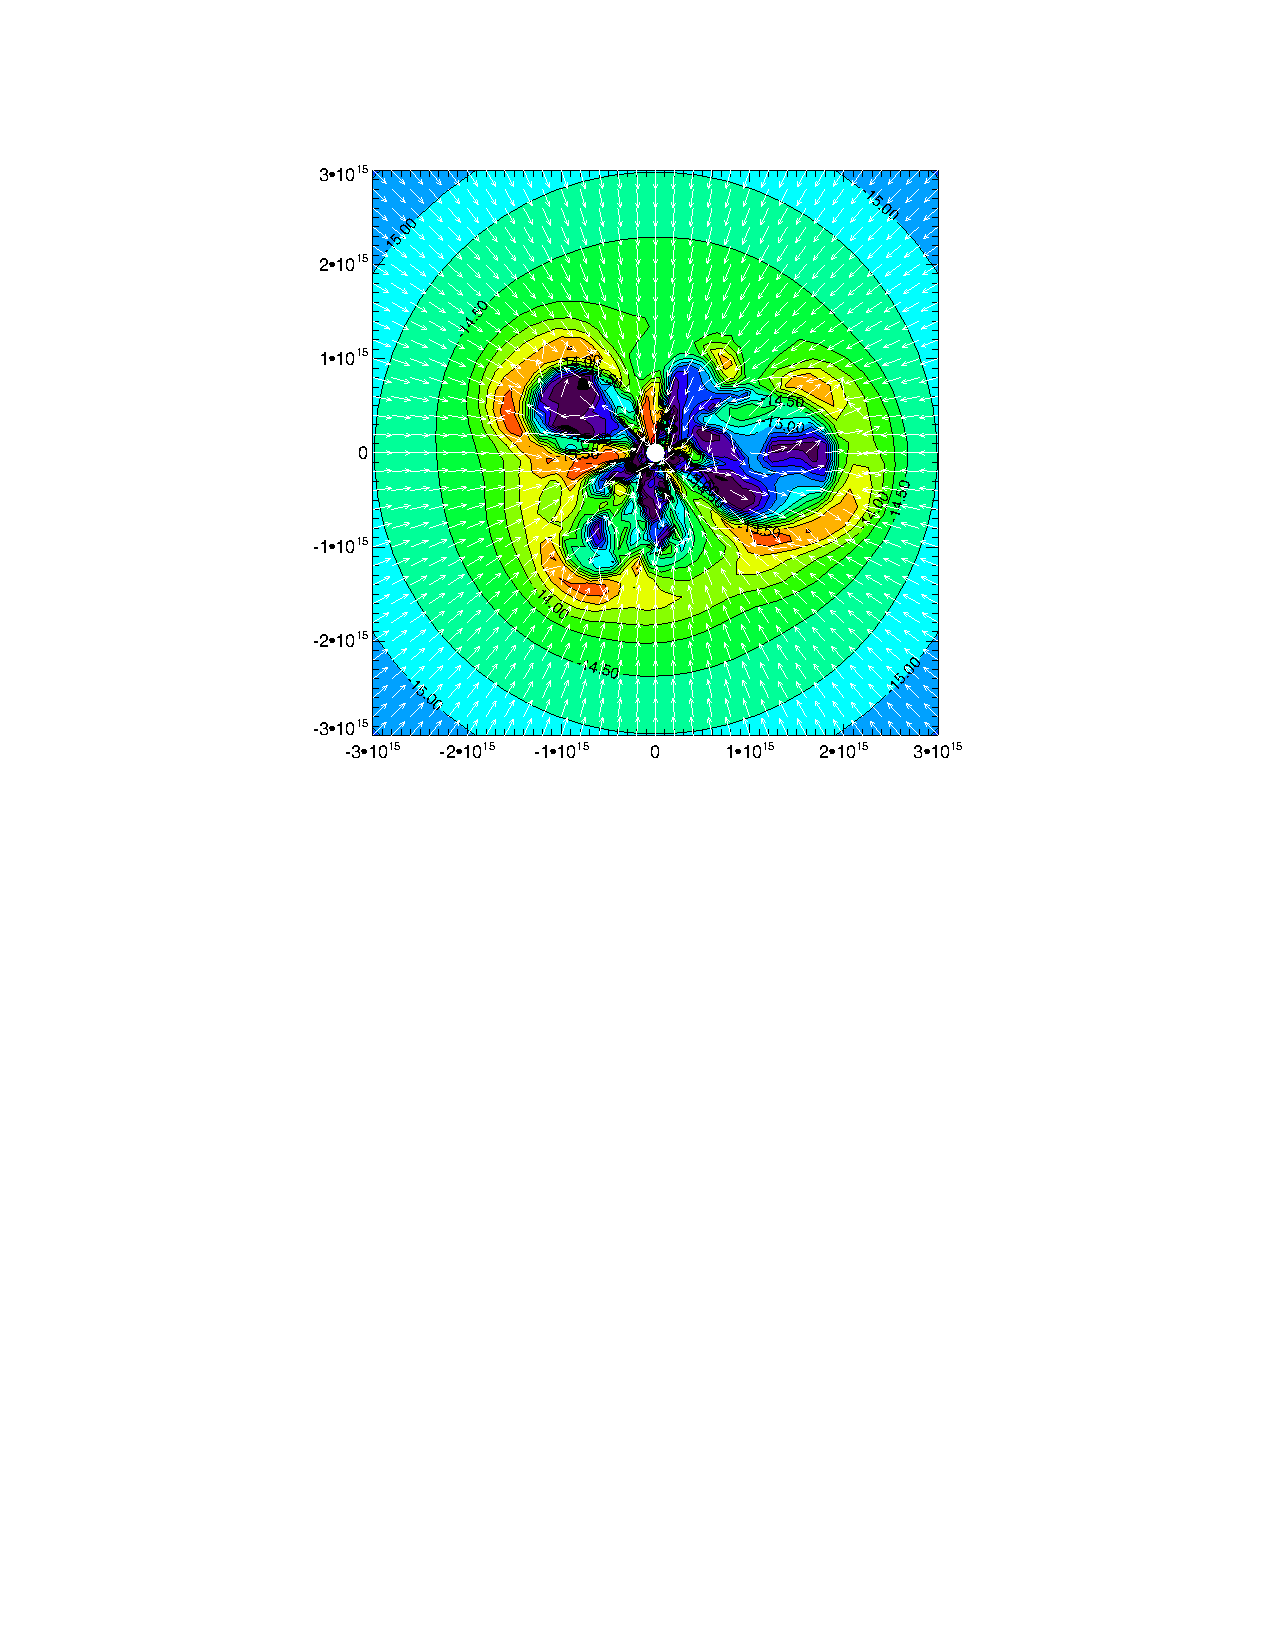
\includegraphics[width=\linewidth]{magdisk_krasnopolsky12}
\caption[Simulations of magnetized rotating collapse with non-ideal MHD]{
\label{fig:magdisk_krasnopolsky12}
Results from a simulation of magnetized rotating collapse including the effects of ion-neutral drift and Ohmic dissipation. Lengths on the axes are in units of cm. Colors and contours show the density in the equatorial plane, on a logarithmic scale from $10^{-16.5}$ to $10^{-12.5}$ g cm$^{-3}$. Arrows show velocity vectors. Credit: \citet{krasnopolsky12a}, \copyright AAS. Reproduced with permission.
}
\end{marginfigure}

\subsection{Steady Thin Disks}

\paragraph{Evolution equations.}

Consider a thin disk of surface density $\Sigma$ orbiting at an angular velocity $\Omega$. We take the disk to be cylindrically symmetric, so that $\Sigma$ and $\Omega$ are functions of the radius $\varpi$ only. We assume it is very thin in the vertical direction, so we only need to solve the equations in the plane $z=0$. In addition to its orbital velocity $v_{\phi}=\varpi\Omega$, the gas has a radial velocity $v_\varpi$, which we assume is much less than $v_{\phi}$. This allows the gas to accrete onto a central object.

For this system, the general equation of mass conservation is
\begin{equation}
\frac{\partial}{\partial t}\rho + \nabla\cdot(\rho \vecv) = \frac{\partial}{\partial t}\rho + \frac{1}{\varpi} \frac{\partial}{\partial \varpi}(\varpi \rho v_\varpi) = 0,
\end{equation}
where we have written out the divergence for cylindrical coordinates, and we have used the cylindrical symmetry of the problem to drop the components of the divergence in the $z$ and $\phi$ directions. Since we have a thin disk, the volume density is $\Sigma \delta(z)$, i.e., it is zero off the plane, infinite in the plane, and integrates to $\Sigma$. Integrating the mass conservation equation over $z$ then immediately gives
\begin{equation}
\frac{\partial}{\partial t}\Sigma + \frac{1}{\varpi} \frac{\partial}{\partial \varpi}(\varpi \Sigma v_\varpi) = 0.
\end{equation}
This equation just says that the change in the surface density at some point is equal to the net rate of radial mass flow into or out of it. It is convenient at this point to introduce the mass accretion rate $\dot{M}=-2\pi \varpi \Sigma v_\varpi$, which represents the rate of inward mass flux across the cylinder at radius $\varpi$. With this definition, the mass conservation equation becomes
\begin{equation}
\label{eq:continuity_disk}
\frac{\partial}{\partial t}\Sigma - \frac{1}{2\pi \varpi} \frac{\partial}{\partial \varpi}\dot{M} = 0.
\end{equation}

Next we can write down the Navier-Stokes equation for the fluid,
\begin{equation}
\rho\left(\frac{\partial}{\partial t}\vecv + \vecv\cdot\nabla\vecv\right) = -\nabla p - \rho\nabla\psi + \nabla\cdot \vecT,
\end{equation}
where $p$ is the pressure, $\psi$ is the gravitational potential, and $\vecT$ is the viscous stress tensor. We choose to write the equation in this form, rather than in the conservative formulation we have used elsewhere in this book, because it makes the dependence on the viscous stress tensor particularly explicit, which will become useful below. Integrating this equation over $z$ gives
\begin{equation}
\Sigma \left(\frac{\partial}{\partial t}\vecv + \vecv\cdot\nabla\vecv\right) = -\nabla P - \Sigma \nabla\psi + \int \nabla\cdot \vecT\,dz,
\end{equation}
where $P$ is the vertically-integrated pressure.

Now consider the $\phi$ component of this equation. This is particularly simple, because all $\phi$ derivatives vanish due to symmetry, and the pressure and gravitational forces therefore drop out. This gives\footnote{Note there is some subtlety here in writing out the gradient of a tensor in cylindrical coordinates. \citet{shu92a} has a useful appendix for vector and tensor operations in non-Cartesian coordinate systems.}
\begin{equation}
\Sigma \left[\frac{\partial}{\partial t} v_\phi + \frac{v_\varpi}{\varpi} \frac{\partial}{\partial \varpi}(\varpi v_\phi)\right] = \int \frac{1}{\varpi^2} \frac{\partial}{\partial \varpi}(\varpi^ 2 T_{\varpi\phi})\,dz.
\end{equation}
If we multiply through by $2\pi \varpi^2$, we obtain
\begin{equation}
2\pi \varpi \Sigma \left(\frac{\partial}{\partial t} j + v_\varpi \frac{\partial}{\partial \varpi}j\right) = \int \frac{\partial}{\partial \varpi}(2\pi \varpi^2 T_{\varpi\phi})\,dz = \frac{\partial}{\partial \varpi} \mathcal{T}
\end{equation}
where we have defined $j=\varpi v_\phi$ as the angular momentum per unit mass of the material and
\begin{equation}
\mathcal{T} = 2\pi \varpi \int \varpi T_{\varpi\phi}\, dz.
\end{equation}
Thus we see that this represents an evolution equation for the angular momentum of the gas. The factor $2\pi \varpi \Sigma$ is just the mass per unit radius in a thin ring, so $2\pi \varpi\Sigma j$ is the angular momentum in the ring.

The quantity $\mathcal{T}$ represents the torque exerted on the ring due to viscosity. This is clear if we examine its components. The viscous stress tensor component $T_{\varpi\phi}$ represents the force per unit area created by viscosity. This is multiplied by $\varpi$, so we have $\varpi T_{\varpi\phi}$, which is just the torque per unit area, since it is a force times a lever arm. Finally, this is multiplied by $2\pi \varpi$ and integrated over $z$, which is just the area of the cylindrical surface over which this torque is applied. Thus, $\mathcal{T}$ is the total torque. We take its derivative with respect to $\varpi$ to obtain the difference in torque between the ring immediately interior to the one we are considering and the ring immediately exterior to it. 

Suppose we look for solutions of this equation in which the angular momentum per unit mass at a given location stays constant, i.e., $\partial j/\partial t=0$. This will be the case, for example, of a disk where the azimuthal motion is purely Keplerian at all times, or more generally for any disk orbiting in a fixed potential. In this case the evolution equation just becomes
\begin{equation}
\label{eq:angmom_disk}
-\dot{M} \frac{\partial j}{\partial \varpi} = \frac{\partial \mathcal{T}}{\partial \varpi}.
\end{equation}
This equation describes a relationship between the accretion rate and the viscous torques in a disk. Its physical meaning is that the accretion rate $\dot{M}$ is controlled by the rate at which viscous torques remove angular momentum from material closer to the star and give it to material further out. 

To make further progress, let us write down the viscous stress $T_{\varpi\phi}$ a little more specifically. We will assume that the gas in the disk is Newtonian, meaning that the viscous stress is proportional to the rate of strain in the fluid. We want to know $T_{\varpi\phi}$, meaning the force per unit area in the $\phi$ direction, exerted on the radial face of a fluid element. Consider an observer in a frame comoving with the orbiting fluid at some particular distance $\varpi$ from the star, and consider a fluid element that is initially on the same radial ray as the observer, but a distance $d\varpi$ further from the star. If the rotation is solid body, then the fluid element and the observer will always lie on the same radial ray, so there is no strain, and there will be no viscous stress. On the other hand, if there is differential rotation, such that the fluid further the star has a longer orbital period (as we expect for Keplerian motion), the fluid element will gradually fall behind the observer. This represents a strain in the fluid.

How quickly does the element fall behind? The difference in angular velocity between the observer and the fluid element is $d\Omega = (d\Omega/d\varpi) d\varpi$, and so the difference in spatial velocity is $\varpi (d\Omega/d\varpi) d\varpi$. The rate of strain is defined as one over the time it takes the fluid element to be displaced a distance $d\varpi$ downstream from the observer, i.e., the time it takes for the differential rotation to stretch the fluid in between by an amount of order unity. Thus, the rate of strain is $\varpi (d\Omega/d\varpi) d\varpi/d\varpi = \varpi (d\Omega/d\varpi)$.

The viscous stress is equal to this rate of strain times the dynamic viscosity $\mu$, so
\begin{equation}
T_{\varpi\phi} = \mu \varpi \frac{d\Omega}{d\varpi} = \rho \nu \varpi \frac{d\Omega}{d\varpi},
\end{equation}
where $\nu=\mu/\rho$ is the kinematic viscosity, which will be more convenient to work with, because it is an intensive quantity that depends on the properties of the fluid but not directly on its density. If we plug this into our definition of the viscous torque, we obtain
\begin{equation}
\label{eq:torque}
\mathcal{T} = 2\pi \varpi \int \varpi T_{\varpi\phi}\, dz = 2\pi \varpi^3 \Sigma \nu \frac{d\Omega}{d\varpi}.
\end{equation}
This combined with the equation giving the relationship between $\dot{M}$ and $d\mathcal{T}/d\varpi$ immediately gives us the accretion rate for any steady disk of known surface density and angular momentum profile $j(\varpi)$.

The most interesting case in star formation is for $j$ and $\Omega$ corresponding to Keplerian rotation, $j=\sqrt{GM_*\varpi}$ and $\Omega=\sqrt{GM_*/\varpi^3}$, where $M_*$ is the mass of the central star.\footnote{If we were interested in galactic disks, we might instead have considered a flat rotation curve, $j\propto \varpi$.} If we now take the continuity equation (\ref{eq:continuity_disk}) and the angular momentum equation (\ref{eq:angmom_disk}), express the torque in terms of $\nu$ using equation (\ref{eq:torque}), and plug in the Keplerian values of $j$ and $\Omega$, a little algebra shows that the resulting equation is
\begin{equation}
\label{eq:disk_keplerian}
\frac{\partial \Sigma}{\partial t} = \frac{3}{\varpi} \frac{\partial}{\partial \varpi} \left[\varpi^{1/2} \frac{\partial}{\partial \varpi}\left(\nu \Sigma \varpi^{1/2}\right)\right],
\end{equation}
and the corresponding equation for the radial drift velocity is
\begin{equation}
v_\varpi = -\frac{3}{\Sigma \varpi^{1/2}} \frac{\partial}{\partial \varpi}(\nu \Sigma \varpi^{1/2}).
\end{equation}

These equations can be solved numerically for a given value of $\nu$, and they can be solved analytically in special cases, but it is useful to examine their general behavior first. First, note that equation (\ref{eq:disk_keplerian}) for the evolution of the surface density $\Sigma$ involves a partial time derivative on the left hand side and a second spatial derivative on the right hand side. This is the form of a diffusion equation; because of the extra factor of $\varpi$ and $\nu$ inside the spatial derivatives, it is a non-linear diffusion equation, meaning that the diffusivity is not constant in space. However, the behavior is qualitatively unchanged by the non-linearity, and the system still behaves diffusively. Thus if we start with a sharply peaked $\Sigma$, say a surface density that looks like a ring, it will spread it out. In fact, the case in which $\nu$ is constant and $\Sigma\propto \delta(\varpi-R_0)$ at time 0 can be solved analytically. The analytic solution is shown in Figure \ref{fig:viscring}.

\begin{marginfigure}
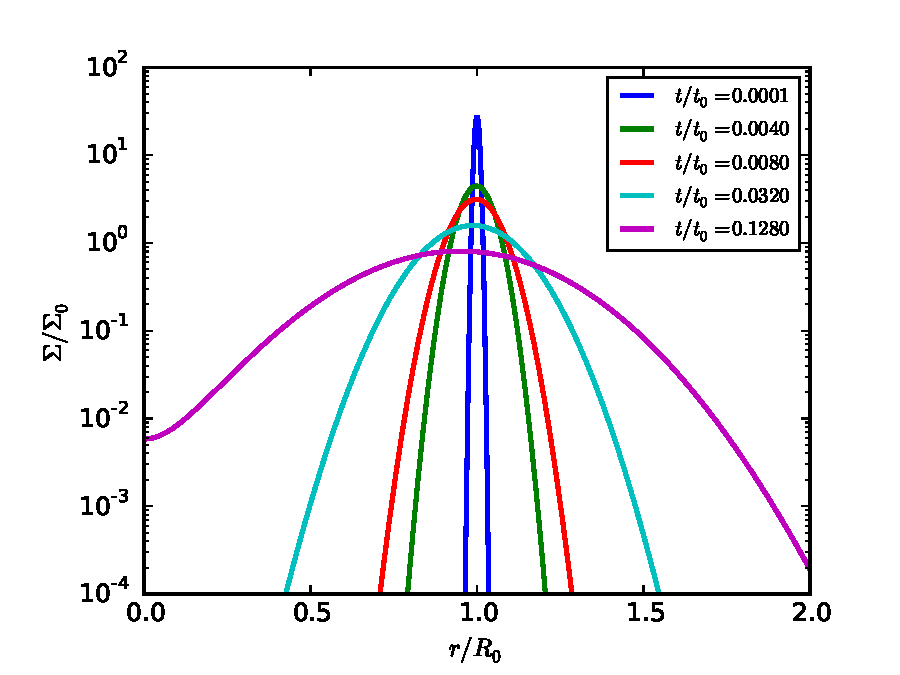
\includegraphics[width=\linewidth]{viscring}
\caption[Viscous ring evolution]{
\label{fig:viscring}
Analytic solution for the viscous ring of material with constant kinematic viscosity $\nu$. At time $t=0$, the column density distribution is $\Sigma = \Sigma_0 \delta(r-R_0)$. Colored lines show the surface density distribution at later times, as indicated in the legend. Times are normalized to the characteristic viscous diffusion time $t_0 = R_0^2/12\nu$. The analytic solution shown is that of \citet{pringle81a}.
}
\end{marginfigure}


How quickly to do rings spread, and does mass move inward? To answer that, we must evaluate $\partial \mathcal{T}/\partial \varpi$ under the assumption that $\Sigma$ and $\nu$ are relatively constant with radius, so we can take them out of the derivative, and that the disk is in steady state. We again assume Keplerian background rotation to evaluate $\Omega$. Under these assumptions
\begin{equation}
\frac{d\mathcal{T}}{d\varpi} = 2\pi \Sigma \nu \frac{d}{d\varpi}\left(\varpi^3 \frac{d\Omega}{d\varpi}\right) = -3\pi\Sigma \nu \frac{d}{d\varpi}(\varpi^2\Omega) = -3\pi \Sigma \nu \frac{dj}{d\varpi},
\end{equation}
and the angular momentum evolution equation (\ref{eq:angmom_disk}) trivially reduces to
\begin{equation}
\dot{M} = 3\pi\Sigma\nu.
\end{equation}
Thus the accretion rate is just proportional to the viscosity and the disk surface density. The radial velocity of the material under these assumptions is
\begin{equation}
v_\varpi = -\frac{3}{2} \frac{\nu}{\varpi}.
\end{equation}
The time required for a given fluid element to reach the star, therefore, is $t_{\rm acc}\sim \varpi/v_\varpi \sim \varpi^2/\nu$.

\paragraph{The $\alpha$ model.}

Before delving into the physical origin of the viscosity, it is helpful to non-dimensionalize the problem. We will write down the viscosity in terms of a dimensionless number called $\alpha$, following the original model first described by \citet{shakura73a}. The model is fairly straightforward. The viscous stress  $T_{\varpi\phi}$ has units of a pressure, so let us normalize it to the disk pressure. This is not as arbitrary as it sounds. If, for example, the mechanism responsible for producing fast angular momentum transport is fluctuating magnetic fields, then we would expect the strength of this effect to scale with the energy density in the magnetic field, which is in turn proportional to the magnetic pressure. Similar arguments can be made for other plausible mechanisms.

The $\alpha$-disk ansatz is simply to set
\begin{equation}
T_{\varpi\phi} = -\alpha p \frac{\Omega/\varpi}{d\Omega/d\varpi},
\end{equation}
where the dimensionless factor $(\Omega/\varpi)/(d\Omega/d\varpi)$ is inserted purely for convenience. This is equivalent to setting
\begin{equation}
\nu = \frac{T_{\varpi\phi}}{\rho \varpi (d\Omega/d\varpi)} = \frac{\alpha c_s^2}{\Omega} = \alpha c_s H,
\end{equation}
where $c_s$ is the sound speed in the disk and $H = c_s/\Omega$ is the disk scale height. Note that $c_s$ and $H$ include both thermal pressure and magnetic pressure. If we now substitute this into our simplified expression for $\dot{M}$, we get an accretion rate
\begin{equation}
\label{eq:mdot_steady}
\dot{M} = 3\pi \Sigma \alpha c_s H = 3\pi \Sigma \alpha \frac{c_s^2}{\Omega}
\end{equation}
Thus if we know the disk thermal structure, i.e.\ we know $c_s$ and $H$, and we know its surface density $\Sigma$, then $\alpha$ tells us its accretion rate.

The physical meaning of this result becomes a bit clearer if we put in an order of magnitude estimate that $\Sigma \approx M_d / R_d^2$, where $M_d$ and $R_d$ are the disk mass and radius. Putting this in we have
\begin{equation}
\dot{M} \approx \alpha \frac{M_d}{R_d^2} \frac{c_s^2}{\Omega}
\end{equation}
If we define $t_{\rm acc} = M_d/\dot{M}$ as the accretion timescale (the characteristic time to accrete the entire disk), $t_{\rm cross} = R_d/c_s$ as the sound crossing time of the disk, and $t_{\rm orb} = 2\pi/\Omega$ as the disk orbital period, then with a little algebra it is easy to show that this expression reduces to
\begin{equation}
t_{\rm acc} = \frac{1}{\alpha} \left(\frac{t_{\rm cross}}{t_{\rm orb}}\right)^2 t_{\rm orb}.
\end{equation}
Thus the time required to drain the disk is of order $(1/\alpha)(t_{\rm cross}/t_{\rm orb})^2$ orbits. Note that $t_{\rm orb} \ll t_{\rm cross}$, because orbital speeds are highly supersonic (as they must be for a thin disk to form). In a disk with $\alpha = 1$, the number of orbits required to drain the disk is this ratio squared, and with $\alpha < 1$ it takes longer, with the number of orbits required scaling as $\alpha^{-1}$. Based on observations of the accretion rates in disks and these properties, \citet{hartmann98a} estimate that $\alpha \sim 10^{-2}$ in nearby T Tauri star disks. It is probably larger at earlier phases in the star formation process.

\subsection{Physical Origins of Disk Viscosity}

We have established that there must be a viscous mechanism to transport angular momentum and mass through accretion disks, and we have even estimated its strength from observations, but we have not yet specified what that mechanism is.

\paragraph{Ordinary fluid viscosity.}

The obvious place to start is to examine the ordinary hydrodynamic viscosity we expect all fluids to have. The kinematic viscosity of a diffuse gas is $\nu = 2\overline{u}\lambda$, where $\overline{u}$ is the RMS particle speed and $\lambda$ is the mean free path. Let us consider a protostellar accretion disk with the typical properties density $n=10^{12}$ cm$^{-3}$ and temperature 100 K. In this case the velocity $\overline{u} = 0.6$ km s$^{-1}$, and assuming a particle-particle cross section of $\sigma=(1\mbox{ nm})^2$, the mean free path is $\lambda \sim 1/(n\sigma)=100$ cm, and $\nu \sim 10^8$ cm$^{-2}$ s. We can put this in terms of $\alpha$ if we remember that $\nu = \alpha (c_s^2/\Omega)$. If the material under consideration is orbiting 100 AU from a 1 $\msun$ star, then $\Omega = 6.3\times 10^{-3}$ yr$^{-1}$, and we have $\alpha \approx 6\times 10^{-12}$.

This is obviously a problem. Suppose the gas starts out $\sim 100$ AU from the star. The time required for the gas to accrete is then $t_{\rm acc}\sim \varpi^2/\nu \sim (100\mbox{ AU})^2/\nu \sim 10^{22}$ s, or just shy of $10^{15}$ yr. In other words, longer than the age of the universe. The obvious conclusion from this is that ordinary hydrodynamic viscosity is completely ineffective at producing accretion. If that were the only source of angular momentum transport in a disk, then stars would never form. Something else must be at work.

\paragraph{Turbulent hydrodynamic viscosity.}

One possible explanation solution to this problem is turbulent hydrodynamic viscosity. If there are large-scale radial motions within a disk, then the effective value of $\overline{u}\lambda$ could be significantly larger than the microphysical one we calculated. In effect, these motions will mix material from different radii within the disk, exchanging angular momentum between inner and outer parts of the disk. This would require the existence of an instability capable of generating and sustaining large radial turbulent motions. Although several such mechanisms have been proposed, it is essentially impossible to determine the amount of angular momentum transport that will be produced based on purely analytic calculations. That is because the transport will depend on the non-linear saturation amplitude of any instability, which is not something that one can generally determine analytically.

Numerical simulations have been attempted, and seem to find that hydrodynamic mechanisms do not produce significant angular momentum transport, but they may be compromised by limited resolution. In a numerical simulation, the maximum possible Reynolds number is set by the ratio of the size of the computational domain to the size of a grid cell, since flows are always smoothed on the grid scale. Even for the largest calculations ever performed this is at most a few thousand, whereas we have seen that the Reynolds numbers in real astrophysical systems are typically $\sim 10^9$. Thus, if the saturation were Reynolds number-dependent, numerical simulations would not get it right.

The question of whether hydrodynamic mechanisms could be responsible for angular momentum transport is sufficiently complex and interesting that the latest frontier is laboratory experiment. Researchers construct counter-rotating cylinders filled with a fluid, and set the cylinders rotating to produce a Keplerian-like rotation profile. They then measure the force exerted on the inner and outer cylinders to measure the rate of angular momentum transport. The laboratory experiments can reach Reynolds numbers of $\sim 10^6$, and seem to find negligible transport, $\alpha < 10^{-6}$ \citep{ji06a}. Given these results, most researchers are convinced that purely hydrodynamic mechanisms cannot explain the observed lifetimes and rates of angular momentum transport in disks. Instead, some other mechanism is required.

\paragraph{Magneto-rotational instability.}

Magnetic fields offer one opportunity for angular momentum transport. We have already mentioned magnetic braking as a possibility, but that requires that the matter be well-coupled to the field, and that the field be dragged inward into the disk so that there is a large net flux. This may not happen due to non-ideal MHD effects, however.

Another mechanism is possible that does not require a large net flux, and that allows weaker (although not zero) coupling. This is the magneto-rotational instability (MRI), first discovered mathematically by \citet{chandrasekhar61a}, and later re-discovered and applied to astrophysical systems by \citet{balbus91a}. The full theory of MRI has been explored extensively both analytically and numerically.

The basic idea is that magnetic field lines threading the disk connect annuli at different radii. As the disk rotates and the annuli shear, this stretches the magnetic field line connecting them. This causes an opposing magnetic tension, which attempts to force the two points to stay close together, and thus to force them into co-rotation. This speeds up the outermost fluid element, which is falling behind, and slows down the innermost one, and thus it moves angular momentum outward. However, when one removes angular momentum from a fluid element it tends to fall toward the center, so the innermost fluid element falls even closer to the star. Similarly, the outermost fluid element gains angular momentum, and so it wants to move outward. This increases the tension even more, and the system goes unstable due to this positive feedback loop.

Simulators are still working to try to come up with a general result about the value of $\alpha$ produced by the MRI, but in at least some cases $\alpha$ as high as $0.1$ seems to be possible. This would nicely explain the observed accretion rates and lifetimes of T Tauri star disks. MRI is not the end of the story, however. The problem with MRI is that it only operates as long as matter is sufficiently coupled to the magnetic field, which in turn depends on its ionization state. MRI will only operate if the mechanism we have described is able to generate turbulent fluctuations in the magnetic field to transport angular momentum. In turn, this requires that no non-ideal mechanism, of which there are several possibilities, be able to smooth out the field over the scale of the accretion disk.

\begin{marginfigure}
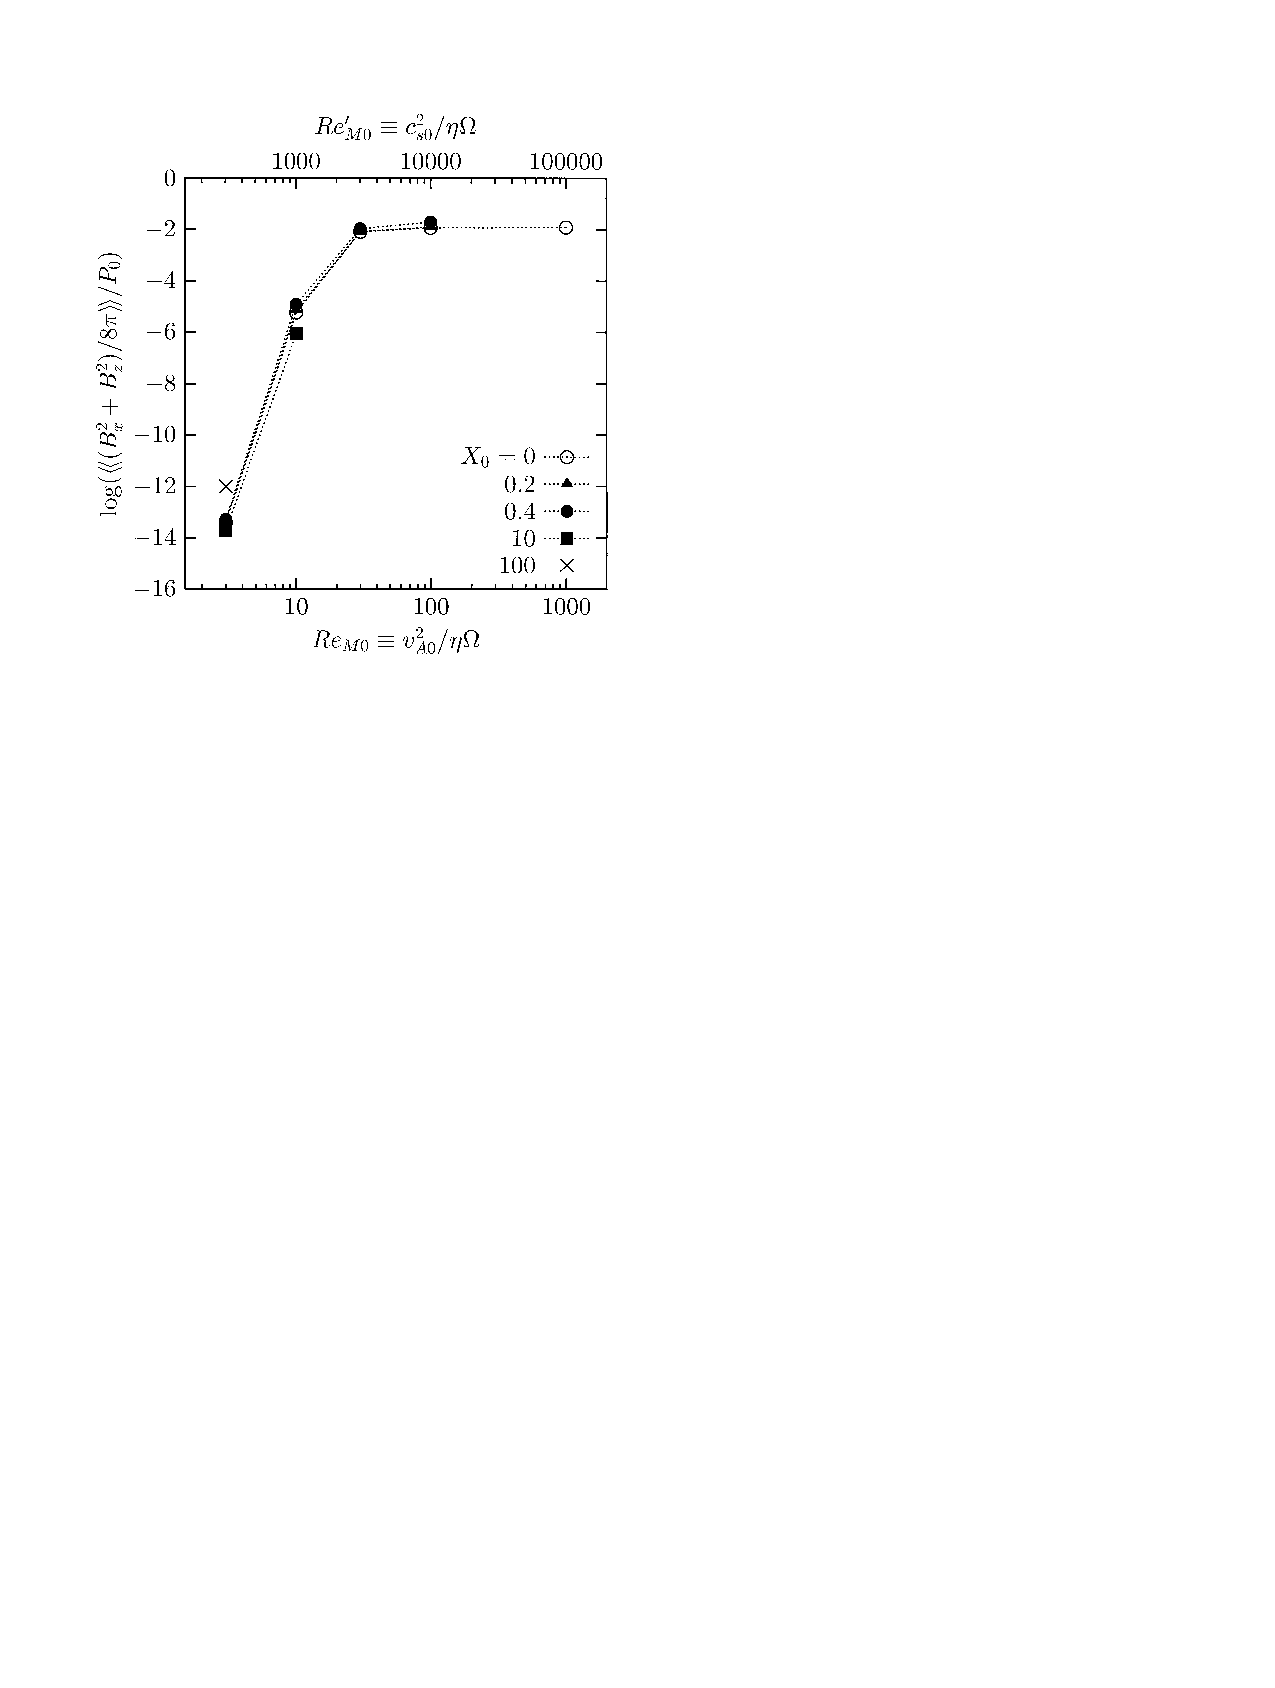
\includegraphics[width=\linewidth]{mri_sano02}
\caption[Maxwell stress in non-ideal MHD simulations of the MRI]{
\label{fig:mri_sano02}
Results from a series of simulation of magneto-rotational instability with non-ideal MHD. The $y$ axis shows the mean Maxwell stress measured in the simulation once it reaches statistical steady state, normalized by the gas pressure. This is roughly the same as $\alpha$. Simulations are shown at a range of magnetic Reynolds numbers $\mbox{Re}_{\mathrm{M}}$. Different values of the parameter $X_0$ correspond to different strengths of Hall diffusivity. Credit: \citet{sano02a}, \copyright AAS. Reproduced with permission.
}
\end{marginfigure}

The question of how well coupled the gas and the field are turns on details of the ionization structure of the disk. Turbulence requires large values of the magnetic Reynolds number $\mbox{Re}_{\rm M} = v_A^2 /(\eta\Omega)$, where $v_A$ is the Alfv\'en speed and $\eta$ is the magnetic diffusivity. Numerical experiments suggest that MRI shuts of when $\mbox{Re}_{\rm M} \lesssim 3000$ (Figure \ref{fig:mri_sano02}). The diffusivity, in turn, depends on the electron fraction: $\eta = c^2/(4\pi \sigma_e)$, where $\sigma_e = n_e e^2/(m_e \nu_c)$ is the conductivity and $\nu_c$ is the frequency of electron-neutral collisions. If there are few electrons, $\sigma_e$ is small and $\eta$ is large, making $\mbox{Re}_{\rm M}$ small. This means that, in order to know where and whether MRI will operate, we need to know the ionization fraction in the disk.

This is an incredibly complex problem, because the ionization is generally non-thermal, non-LTE, and it only takes a tiny number of electrons to make MRI operate: an electron fraction $\sim 10^{-9}$ is sufficient. In the very inner disk near the star, where the temperature is $\sim 2000$ K, thermal ionization of alkali metals will provide the necessary electrons. In regions where the disk column density is $\lesssim 100$ g cm$^{-2}$, X-rays from the central star and cosmic rays can penetrate the disk, providing free electrons. However, for comparison the estimated column density of the minimum mass Solar nebula (the minimum mass required to make all the planets -- to be discussed further in Chapter \ref{ch:late_disk}) is 1700 g cm$^{-2}$ at 1 AU, and the equilibrium temperature is $\ll 2000$ K.

In such high column density, cool regions, the electron fraction depends on such complex questions as the mean size of dust grains (since these can absorb free electrons) and the rate of vertical transport of electrons from the surface layers down to the disk midplane. One possible result of this is that MRI would operate only at the surface of disk, leaving the midplane a ``dead zone". Another possibility is that there may be radial dead zones with no MRI. Material would move inward to such regions, but then get stuck there, potentially making accretion bursty.

\paragraph{Gravitational transport mechanisms.}

Magnetic fields provide on potential source of transport, but, as we have seen, they may fail if the gas is not sufficiently ionized. If the accretion rate onto the disk is large enough, it is also possible that MRI may operate, but may not provide sufficiently rapid angular momentum transport to stop gas from building up the disk -- this is likely to occur particularly for massive stars. In this case, mass can build up in the disk, leading to gravitational instability.

We can understand when gravitational instability is likely to set in using our theory of disks. In steady state we showed that the accretion rate depends on $\Sigma$, $\alpha$, $c_s$, and $\Omega$ (equation \ref{eq:mdot_steady}). Since we are interested in gravitational stability, let us introduce the Toomre $Q$ parameter for our disk,
\begin{equation}
Q = \frac{\Omega c_s}{\pi G \Sigma}
\end{equation}
where we have $\Omega$ rather than $\sqrt{2}\Omega$ because the rotation curve is Keplerian rather than flat as in a galactic disk, and where we are assuming the non-thermal velocity dispersion in the disk is subsonic. Solving for $\Sigma$ in terms of $Q$ and inserting the result into equation (\ref{eq:mdot_steady}), we obtain
\begin{equation}
\dot{M} = \frac{3\alpha}{Q} \frac{c_s^3}{G}.
\end{equation}

Thus we see that, if $Q > 1$, so the disk is gravitationally stable, and $\alpha < 1$, as we expect for MRI or almost any other local transport mechanism, the maximum rate at which the disk can move matter inward is roughly $c_s^3/G$. This is also the characteristic rate at which matter falls onto the disk from a thermally-supported core, provided that we use the sound speed in the core rather than in the disk.

Normally disks are somewhat warmer than the cores around them, both because the star shines on the disk and because viscous dissipation in the disk releases heat. However, what this result shows is that, in any regions where the disk is not significantly warmer than the core that is feeding it, for example the outer parts of the disk where stellar and viscous heating are small, the disk cannot transport matter inward as quickly as it is fed. The result will be that the surface density will rise and $Q$ will decrease, giving rise to gravitational instability.

This can in turn generate transport of angular momentum via gravitational torques. Transport of this sort comes in two flavors: local and global. Local instability happens when the disk clumps up on small scales due to its own gravity. This depends on the Toomre $Q$ of the disk. If $Q\sim 1$ it will begin to clump up, and these clumps can transport angular momentum by interacting with one another gravitationally, sending mass inward and angular momentum outward. However, this clumping will heat the gas via the release of gravitational potential energy, which in turn tends to drive $Q$ back to higher values.

What happens then depends on how the gas radiates away the excess energy. If the radiation rate is too low, the gas will heat up until it smoothes out, and the Toomre $Q$ will be pushed up. If it is too high, the gas will fragment entirely and collapse into bound objects in the disk -- something like what happens in a galactic disk. If it is in between, the disk can enter a state of sustained gravitationally-driven turbulence in which there is no fragmentation but the rate of heating by compression balances the rate of radiation, and there is a net transport of mass and angular momentum.

The global variety of gravitational instability occurs when the disk clumps up on scales comparable to the entire disk. This occurs when the disk mass becomes comparable to the mass of the star it is orbiting; instability sets in at disk masses of $30-50\%$ of the total system mass. This generally manifests as the appearance of spiral arms. These instabilities transport angular momentum because the disk is no longer axisymmetric, and instead has a significant moment arm that can exert torques, or on which torques can be exerted. Transport of angular momentum can then occur in several ways. If there is an envelope outside the disk, the disk can spin up the envelope, sending angular momentum outward in that way.

The disk can also transfer angular momentum to the star by forcing the star to move away from the center of mass. In this configuration the disk develops a one-armed spiral, and the star in effect goes into a binary orbit with the overdensity in the disk. In this case angular momentum is transported inward rather than out, with the excess angular momentum going into orbital motion of the star. This phenomenon is known as the Sling instability \citep{shu90a}.

\section{Outflow Launching}

The final topic for this chapter is how and why disks launch the ubiquitous jets and winds that observations reveal. The topic of jets is not limited to the star formation context, of course, and much of the theory for it was originally developed in the context of active galactic nuclei and compact objects. We will only scratch the surface of this theory here. Our goal is just to get a general understanding of how and why we expect winds to be launched from disks, and what general properties we expect them to have.

\subsection{Mechanisms}

We begin by considering what mechanisms could be responsible for launching winds. We can start by discarding the two mechanisms that we usually invoke to explain the winds of main sequence stars. All main sequence stars, including the Sun, produce winds. For low mass stars like the Sun, the driving mechanism is thermal. MHD waves propagating into the low-density solar corona heat the gas to temperatures of up to $\sim 10^6$ K. The high pressure in the hot region drives flows of gas outward; for the Sun, the mass loss rate is roughly $10^{-14}$ $\msun$ yr$^{-1}$, and the mechanical luminosity is $\sim 10^{-4}$ $\lsun$. In contrast, the mechanical power input required to explain the observed outflows from young stars is closer to $\sim 0.1$ $\lsun$. This is far greater than the thermal energy available in the hot X-ray corona of the star -- a corona capable of providing this much power would exceed the total stellar bolometric output.

For massive main sequence stars, the main driving mechanism is the pressure exerted by stellar photons on the gas. The problem with this mechanism is the momentum budget. Observed outflow momentum is generally $1-2$ orders of magnitude larger than $L/c$, the amount of momentum available in the stellar radiation field. In contrast, for the winds of main sequence stars the outflow momentum flux is always $\lesssim L/c$. Thus the stellar photon field does not have enough momentum to drive the observed outflows of young stars. Moreover, neither the thermal winds of low mass main sequence stars, nor the radiatively-driven winds of massive ones, show highly collimated features like the HH jets.

Having discarded these two mechanisms, we must seek an alternative source of energy. The most natural one is the gravitational potential energy being liberated by the accretion flow, which, combined with magnetic fields, can produce highly collimated outflows. The question then becomes exactly how the combination of gravitational power and magnetic fields produces the observed outflows.

\subsection{Stability Analysis for Magnetocentrifugal Winds}

There are a range of theoretical models for the exact mechanism by which winds are launched. However, the general picture of all of these mechanisms is to combine centrifugal force with magnetic fields. Consider a disk of material in Keplerian orbit, and consider an open field line passing through the disk; here by "open" we mean that the field line does not loop back into the disk, but instead goes out, formally to infinity. We write the field in the vicinity of the disk as the sum of a poloidal and a toroidal component,
\begin{equation}
\vecB = \vecB_p + B_\phi \hat{e}_\phi
\end{equation}
The field exerts negligible forces within the disk, but for the much lower-density region above the disk (the corona), magnetic forces are non-negligible.

Let us consider a test fluid element that is, for whatever reason, lofted slightly above the disk, into the corona. We will assume ideal MHD, so the fluid element is constrained to move only along the field line. We can think of the test fluid element as a bead stuck on a wire. We will further assume that the density of material above the disk is very small, so that magnetic forces dominate and the field simply rotates as a rigid body. Now let us consider how this fluid element will evolve in time.

In a frame co-rotating with the launch point of the fluid element, there are two potentials to worry about: the gravitational potential of the central star, and the centrifugal potential that arises from the fact that we have chosen to work in a rotating reference frame. The former is simply the usual
\begin{equation}
\psi_{g} = -\frac{GM_*}{\sqrt{\varpi^2 + z^2}},
\end{equation}
where $M_*$ is the star's mass, and we are working in cylindrical coordinates. For the latter, we are working in a frame rotating at an angular velocity equal to the Keplerian value at the fluid element's launch point $\varpi_0$, which is $\Omega = \sqrt{GM_*/\varpi_0^3}$. The centrifugal potential is therefore
\begin{equation}
\psi_c = -\frac{1}{2}\Omega^2 \varpi^2 = -\frac{1}{2} G M_* \frac{\varpi^2}{\varpi_0^3}.
\end{equation}
Thus the total potential is
\begin{equation}
\psi = -\frac{GM_*}{\varpi_0} \left[\frac{1}{2}\left(\frac{\varpi}{\varpi_0}\right)^2 + \frac{\varpi_0}{\sqrt{\varpi^2+z^2}} \right].
\end{equation}

To determine the evolution of the test fluid element, we must consider the forces associated with this potential. The force per unit mass  is simply minus the gradient of the potential, and thus we have
\begin{equation}
\mathbf{f} = -\nabla \psi = -GM_* \left\{ \varpi \left[\frac{1}{(\varpi^2+z^2)^{3/2}} - \frac{1}{\varpi_0^3}\right]\hat{e}_\varpi + \frac{z}{(\varpi^2+z^2)^{3/2}} \hat{e}_z \right\}
\end{equation}
If we plug in our starting point, $\varpi = \varpi_0$ and $z=0$, we see that the gradient is exactly zero, which is what we expect: the starting point is, by assumption, in equilibrium between centrifugal and gravitational forces.

Now let us consider our perturbed fluid element. It has been moved a distance $ds$ from its starting point, and it is moving along the field line, which has radial and vertical components $B_\varpi$ and $B_z$. For convenience, let us define the angle of the field line relative to the horizontal by
\begin{equation}
\cos \theta = \frac{B_\varpi}{\sqrt{B_\varpi^2 + B_z^2}}.
\end{equation}
An angle $\theta=90^\circ$ corresponds to a field line that has zero radial component, and $\theta=0^\circ$ corresponds to one that has zero vertical component. The coordinates of the displaced fluid element is $\varpi = \varpi_0 + \cos\theta \, ds$ and $z = \sin\theta \, ds$. To determine the force experienced by the fluid element, we simply plug these coordinates into $\mathbf{f}$ and expand to first order:
\begin{equation}
d\mathbf{f} = \frac{GM_*}{\varpi_0^3} \left(3 \cos\theta\,\hat{e}_\varpi - \sin\theta\,\hat{e}_z\right) ds.
\end{equation}

We are interested in the component of this force parallel to the field line, since the fluid element is constrained to move along the field line. That is, we are interested in
\begin{equation}
df_\parallel = d\mathbf{f} \cdot (\cos\theta\,\hat{e}_\varpi +  \sin \theta\,\hat{e}_z) = \frac{GM_*}{\varpi_0^3} \left(3\cos^2 \theta - \sin^2 \theta\right) ds.
\end{equation}
The force is therefore positive, indicating that it is pushing the fluid element further away from the launch point, if
\begin{equation}
3 \cos^2 \theta - \sin^2 \theta > 0
\qquad\Longrightarrow\qquad
\theta < 60^\circ.
\end{equation}
We have therefore derived a condition under which a disk threaded by open field lines will be unstable to the formation of a wind. If the field lines make an angle of $<60^\circ$ off the plane, then any fluid element that is lofted infinitesimally above the disk will be forced further down the field line by the centrifugal force, forming a wind.

\subsection{Properties of the Wind}

If the disk is unstable to wind formation, the next question is what properties that wind will have. We can answer this question at least approximately from the following elementary consideration. We have thus far assumed that the field lines above and below the disk are perfectly rigid, but of course that cannot be strictly true out to infinite radius. If we choose a large enough radius, then maintaining perfect solid body rotation would require a velocity larger than the speed of light, which is obviously forbidden by relativity. However, there is an even more restrictive limit: the field line can remain rigid only as long as the matter attached to it has negligible inertia. If the inertia of the material is significant, it will slow down the field lines, causing them to deviate from rigid rotation.

Recalling our dimensional analysis of the MHD equations in Chapter \ref{ch:turbulence}, the relative importance of the terms describing inertia and magnetic force is determined by the Alfv\'en Mach number,
\begin{equation}
\mathcal{M}_A \sim \frac{v}{v_A},
\end{equation}
where $v_A = B/\sqrt{4\pi \rho}$ is the Alfv\'{e}n speed. The material starts at zero velocity, and accelerates as it moves outward, so that $\mathcal{M}_A$ increases along any given field line. We expect that the field lines will cease to be rigid once the material along them is accelerated to a velocity such that $\mathcal{M}_A \sim 1$. This transition between sub- and super-Alfv\'{e}nic motion will occur at a critical radius $\varpi_A$ (which is not necessarily the same along every field line), called the Alfv\'{e}n radius.

Once the field line starts to unwind at $\varpi_A$, it will no longer be able to impart significant angular momentum or energy to the fluid parcels that travel along it. Returning to our bead on a wire analogy, it is as if the rigid wires that are accelerating the beads are beginning to bend. We therefore expect the terminal velocity of the wind to be of order the wind speed at $\varpi_A$, which is
\begin{equation}
v_\infty \sim \Omega_0 \varpi_A \sim v_{K,0} \frac{\varpi_A}{\varpi_0},
\end{equation}
where $\Omega_0$ is the angular velocity at the launch point, and $v_{K,0}$ is the Keplerian velocity at that point. Thus the wind speed is comparable to the Keplerian speed times a factor of order the ratio of the Alfv\'{e}n radius to the launch radius.

The specific angular momentum of the material ejected in the wind will be
\begin{equation}
j_w \sim \varpi_A v_\infty \sim v_{K,0} \frac{\varpi_A^2}{\varpi_0}.
\end{equation}
For comparison, the specific angular momentum of the material that remains in the disk is
\begin{equation}
j_d = v_{K,0} \varpi_0.
\end{equation}
Thus the specific angular momentum of wind material exceeds that of disk material by a factor of
\begin{equation}
\frac{j_w}{j_d} \sim \left(\frac{\varpi_A}{\varpi_0}\right)^2.
\end{equation}
One factor of $\varpi_A/\varpi_0$ comes from the greater level arm of the material being launched into the wind, and the second factor comes from the greater velocity.

If the wind is predominantly responsible for removing the angular momentum of the disk and allowing accretion, this implies that the rates of mass accretion $\dot{M}$ and wind launch $\dot{M}_w$ must be related by
\begin{equation}
\dot{M} \sim \left(\frac{\varpi_A}{\varpi_0}\right)^2 \dot{M}_w.
\end{equation}
Thus wind launching provides an efficient means to allow accretion, since for even a relatively modest Alfv\'{e}n radius, say $\varpi_A/\varpi_0 \sim 3$, it will enable accretion to occur using only $\sim 1/10$ of the available accreting mass. Of course we have not self-consistently calculated $\varpi_A$, and we will not do so here. Schematically, one must do so by taking a wind mass launching rate (called the mass loading) as a function of radius, and then self-consistently solving for the structure of the magnetic field and the velocity above the disk. The Alfv\'{e}n radius then appears as a critical point of the solution along each streamline / magnetic field line. The first such self-consistent calculation was provided by \citet{blandford82a}, although this calculation still had to leave the mass loading as a free parameter.


